\documentclass[11pt, dvipdfmx, openany]{jsbook}
\usepackage[dvipdfmx]{graphicx}
\usepackage{hyperref}
\usepackage{pxjahyper}
\usepackage[a4paper]{geometry}
\usepackage{amsmath,amssymb}
\usepackage{amsfonts}
\usepackage{algorithm}
\usepackage{algpseudocode}
\usepackage{bm}
\usepackage{here}
\usepackage{color}
\usepackage[hang,small,bf]{caption}
\usepackage[subrefformat=parens]{subcaption}
\hypersetup{colorlinks=false, hidelinks}
\newcommand{\red}[1]{\textcolor{red}{#1}}
\renewcommand{\baselinestretch}{1.1}
\captionsetup{compatibility=false}
\usepackage{url}

\setlength{\textwidth}{\fullwidth}  %本文の幅(textwidth)を全体の幅(=ヘッダ部の幅)にそろえる
\setlength{\evensidemargin}{\oddsidemargin} %偶数ページの余白と奇数ページの余白をそろえる

\begin{document}
\title{2048の研究}
\author{山下修平}
\maketitle 

\tableofcontents
\clearpage

% 本文
\chapter{はじめに}
\chapter{2048}

\section{2048のルールと用語説明}
\label{sec:rule}
2048は, Gabrirle Cirulliによって公開された$1$人用のパズルゲームである~\cite{2048}.
ゲームは$16$マスからランダムに選ばれた$2$マスに$2$か$4$の数字タイルが置かれた盤面から始まる.
プレイヤが行うことは上下左右いずれかの方向を選択することである. 
プレイヤがある$1$つの方向を選ぶと, 盤面上のすべての数字タイルは選択した方向に向かってスライドして移動する.
スライドする数字タイルは空きマスを通過し, 異なる数字タイルの直前か盤面の端で停止する.
スライドして移動する際に$2$つの同じ数字のタイルが衝突すると, これらは合体してその合計の数字の$1$つのタイルへ変化し, プレイヤはその数値を得点として獲得する.
そのため, ゲームには$2$の累乗の数字タイルしか現れない.
図~\ref{fig:all_directions}にある盤面から上下左右を選択したときの, 数字タイルのスライドの仕方の具体例を示す.
\begin{figure}[t]
    \centering
    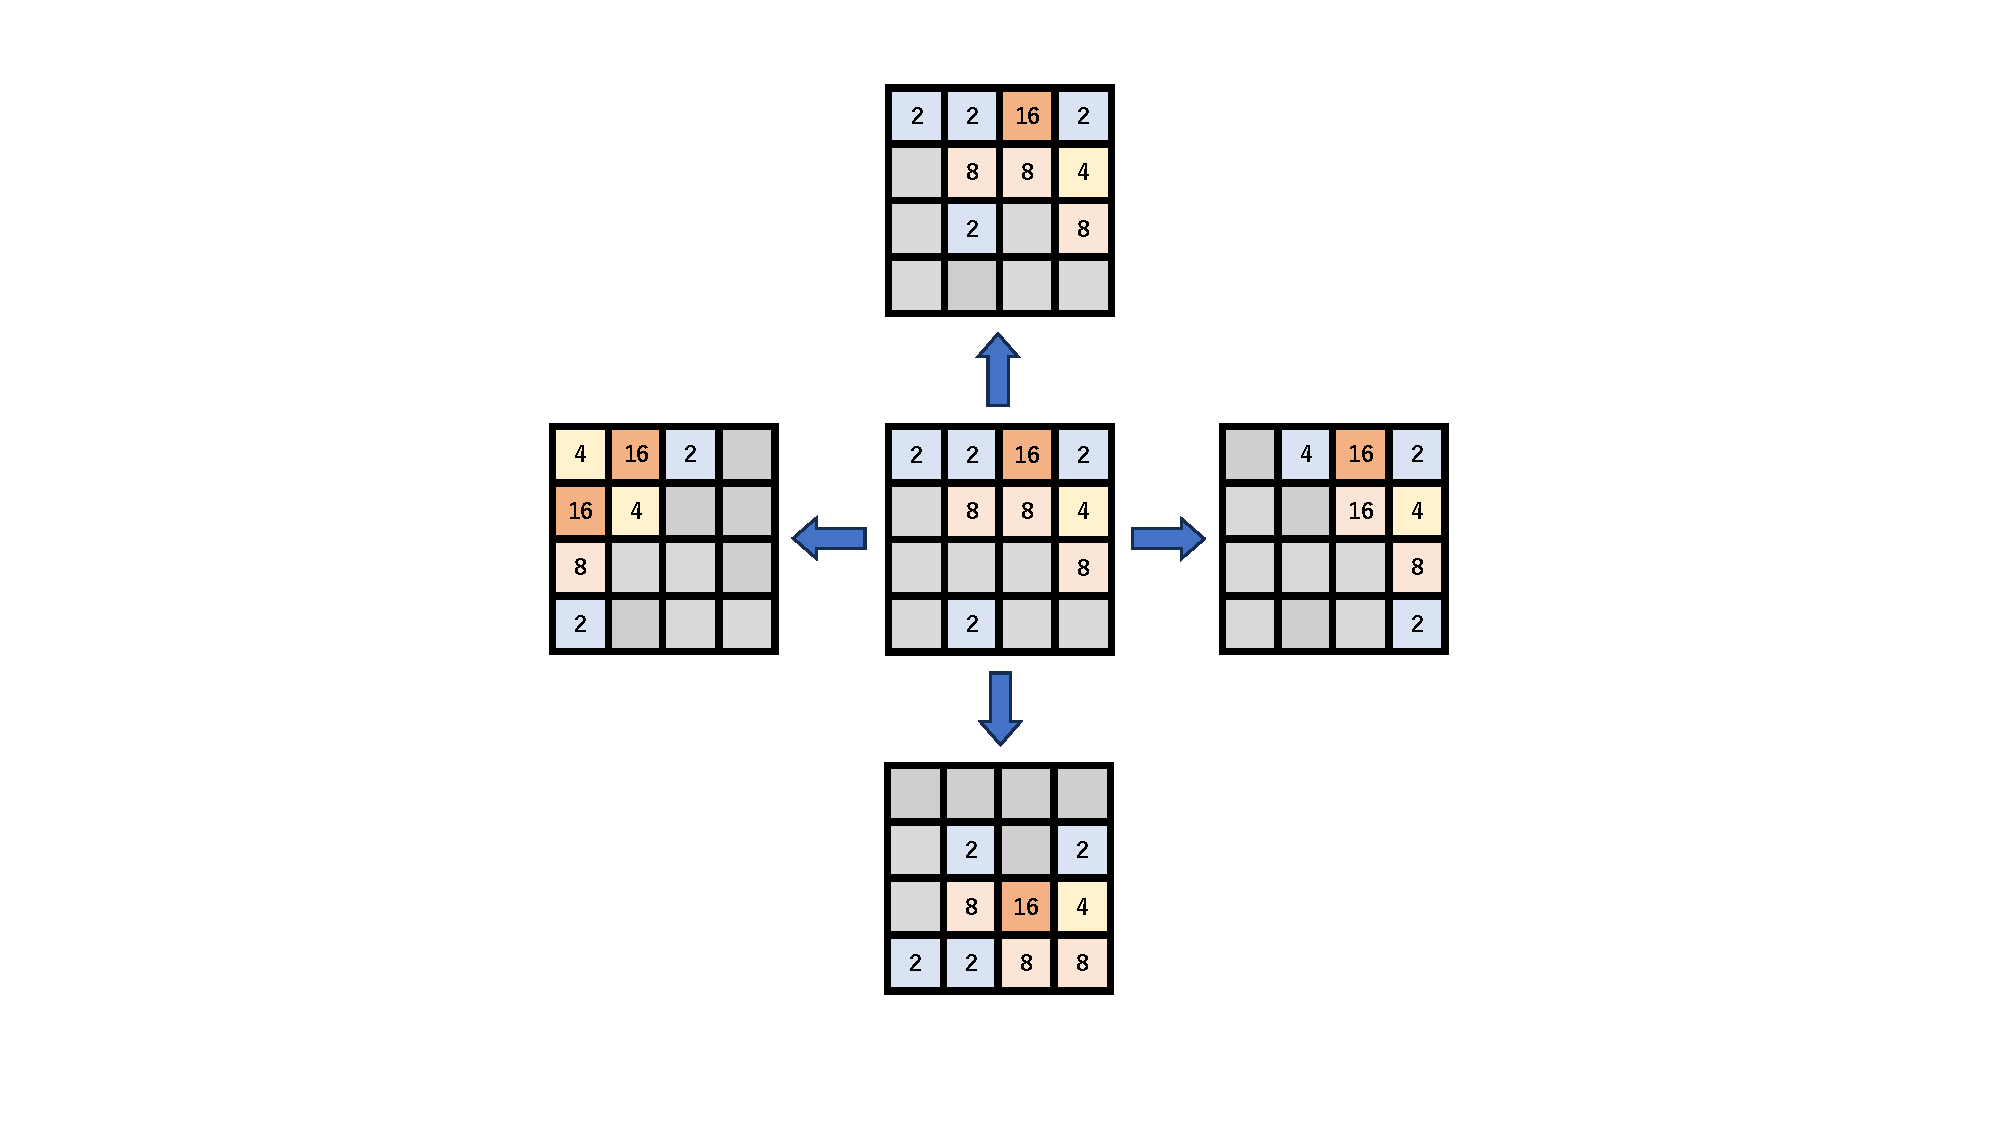
\includegraphics[width=0.8\linewidth{}]{figures/all_directions.pdf}
    \caption{上下左右それぞれへのスライドの例 \label{fig:all_directions}}
\end{figure}

数字タイルのスライド後, 空きマスから等確率に選択されたある1マスに$90\%$の確率で$2$のタイルが, $10\%$の確率で$4$のタイルが置かれる. 
ゲームはプレイヤの行動による数字タイルのスライドと新たな数字タイルの出現を交互に繰り返して進行する.
盤面上の数字タイルが市松模様のようになると, プレイヤが選択可能な行動がなくなったときにゲームは終了する~(図~\ref{fig:terminal}を参照).
\begin{figure}[t]
    \centering
    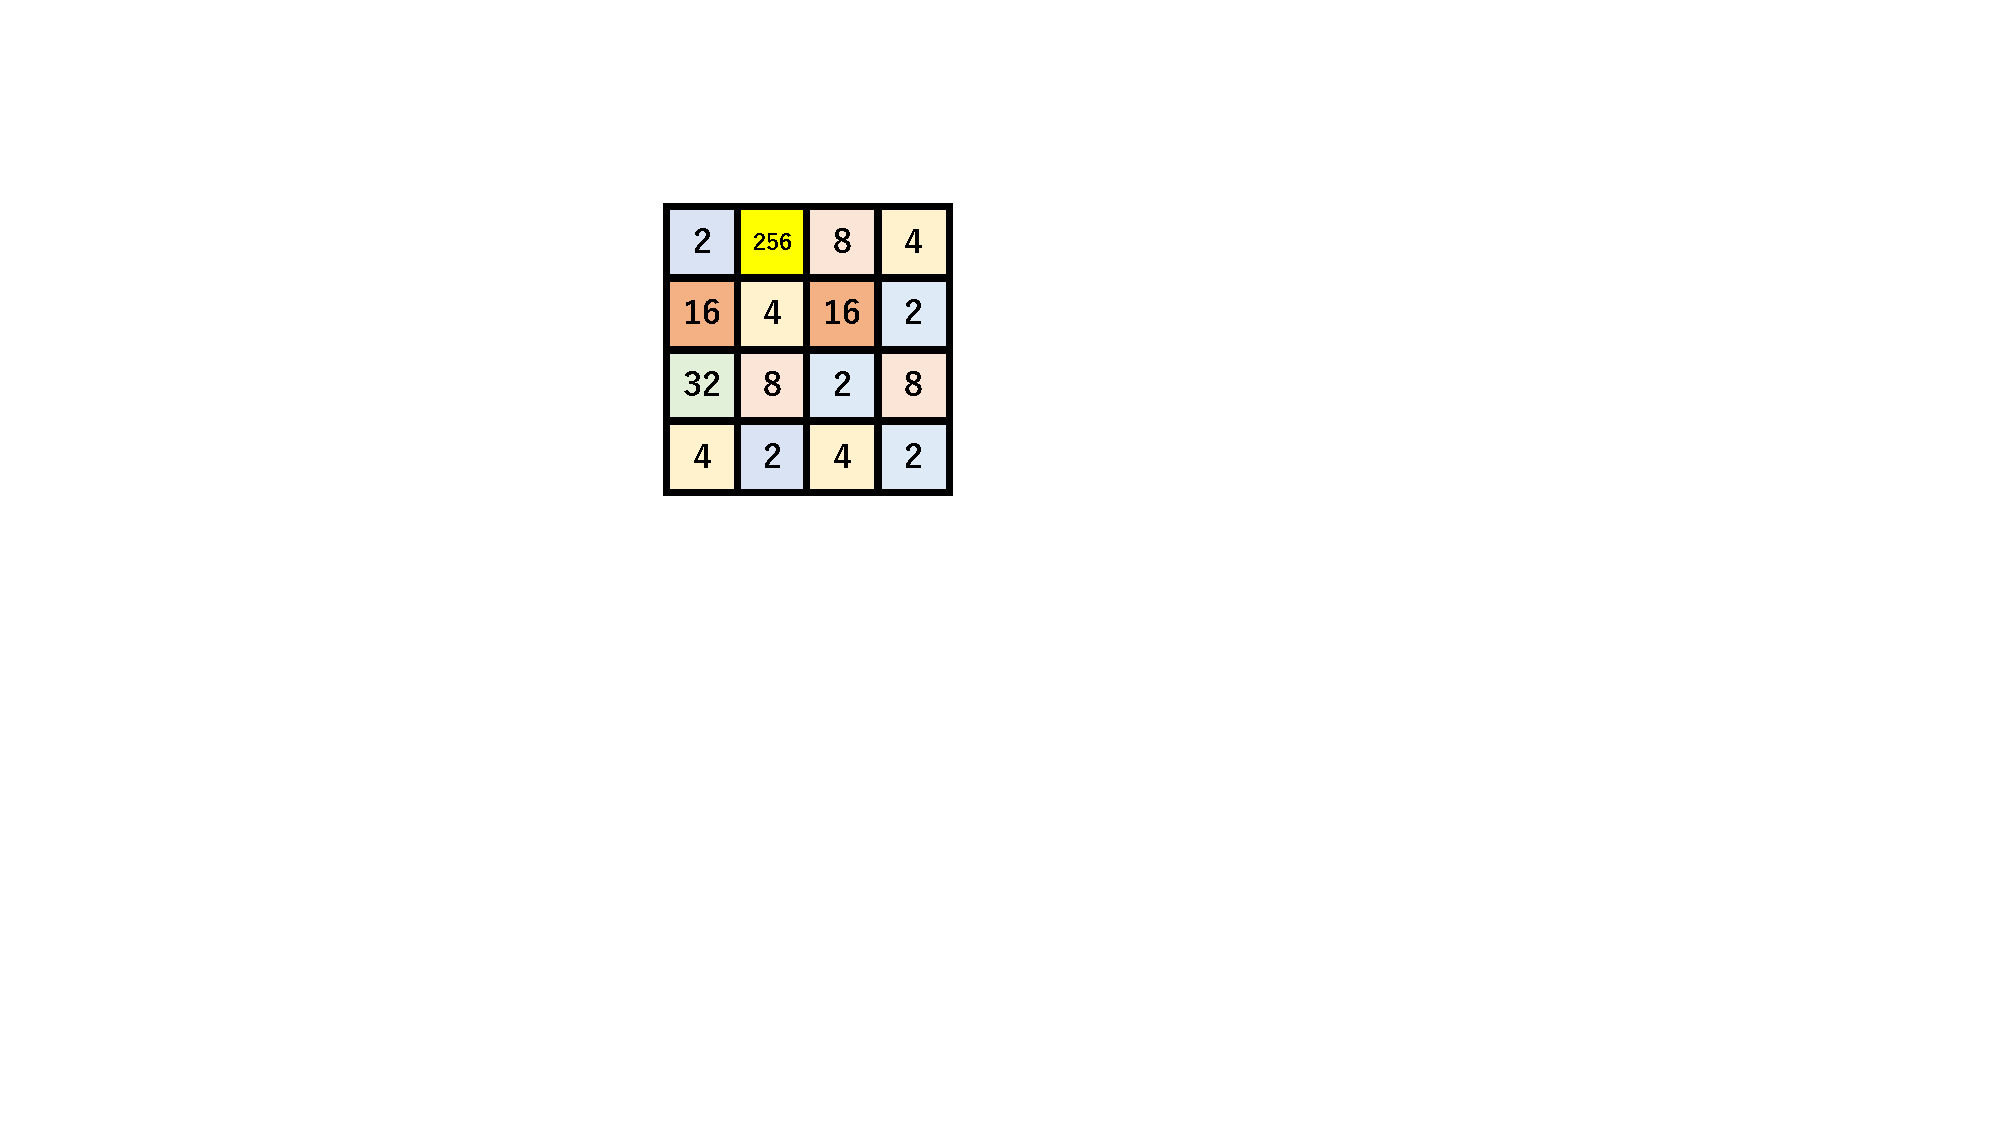
\includegraphics[width=0.2\linewidth{}]{figures/terminal_.pdf}
    \caption{終了状態の例 \label{fig:terminal}}
\end{figure}

ここでプレイヤが行動を選択する盤面を\textgt{状態}, 行動を選択して新たな数字タイルが出現する直前の盤面を\textit{afterstate}と呼ぶ.
図~\ref{fig:transition}に状態$s$からafterstate $s'$を経由して, 次の状態$s_{\text{next}}$に遷移する例を示す.

\begin{figure}[t]
    \centering
    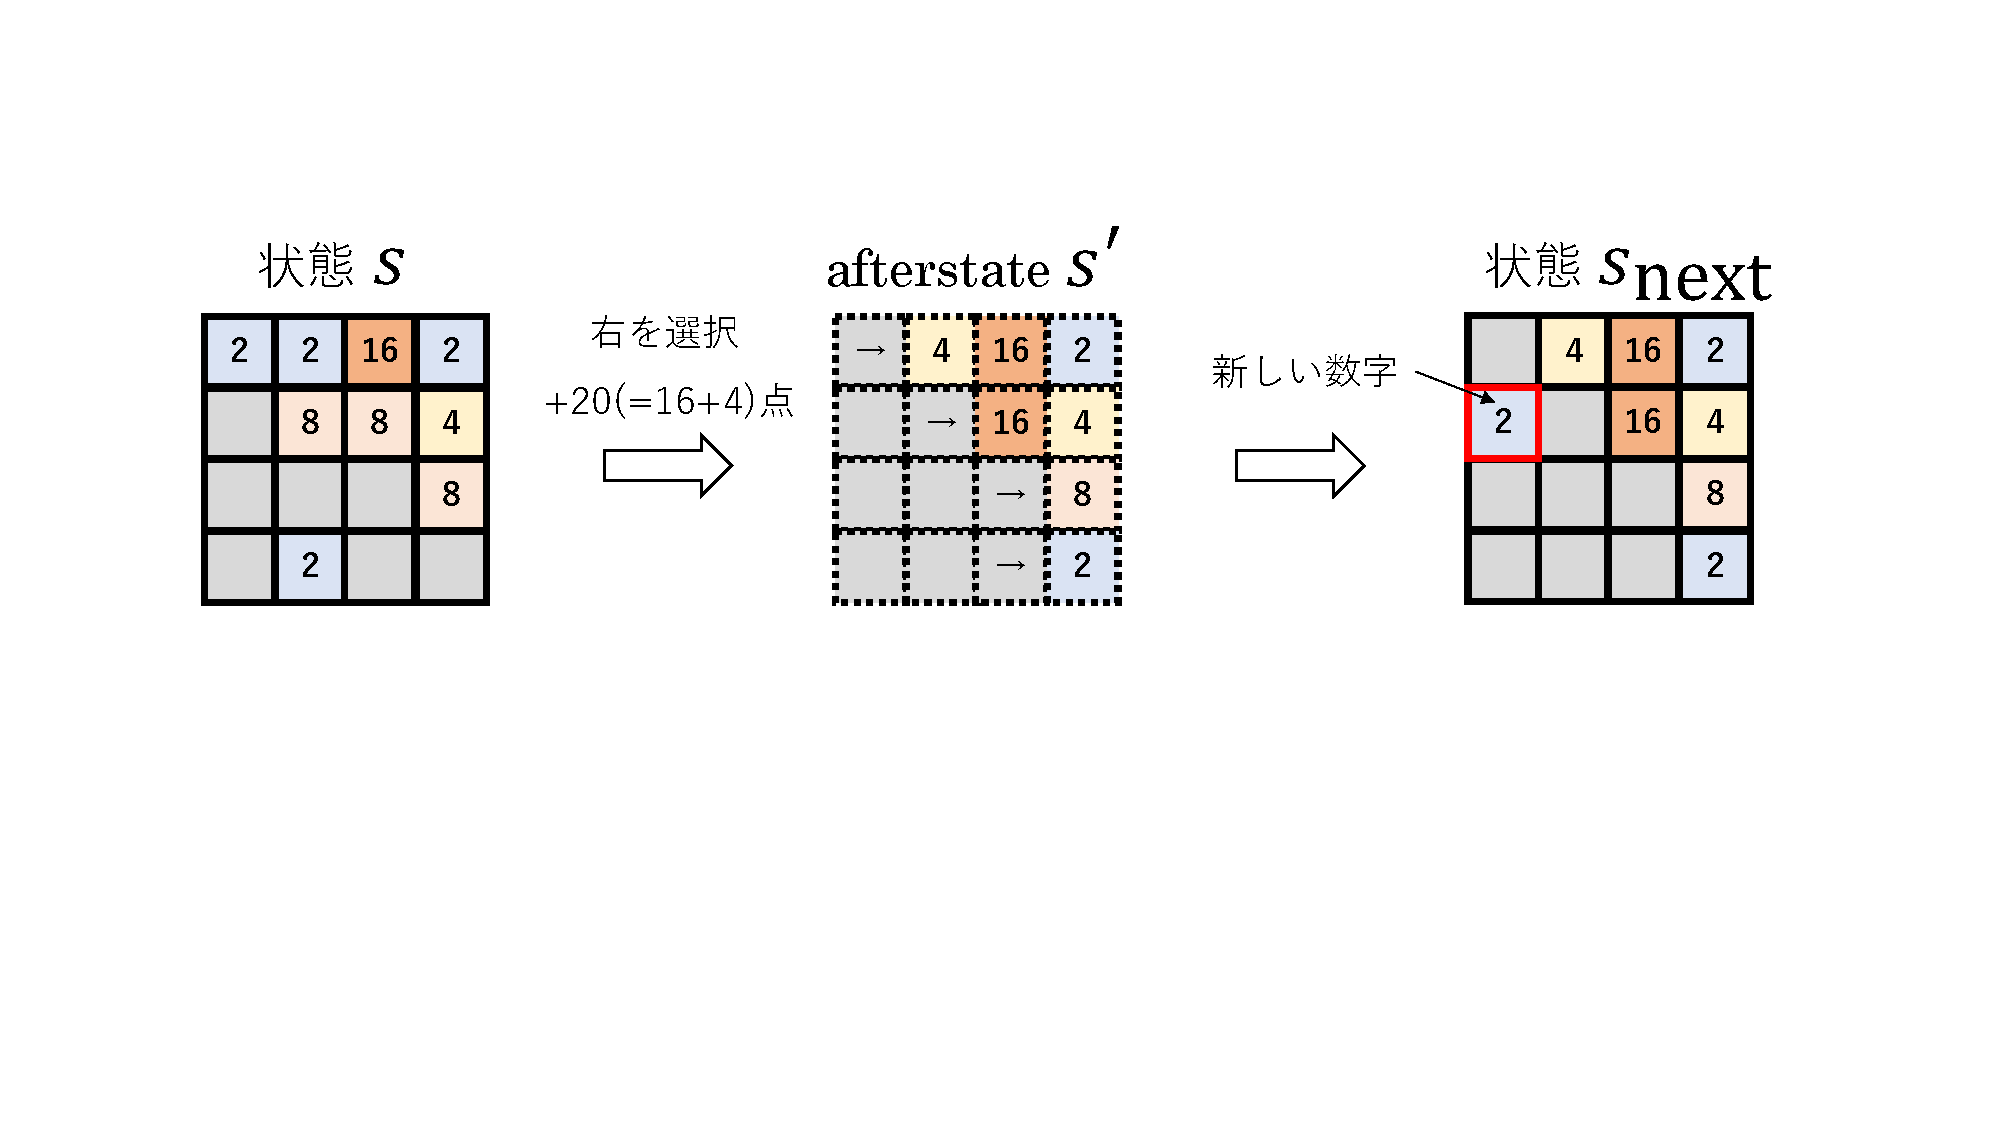
\includegraphics[width=\linewidth{}]{figures/transition_.pdf}
    \caption{状態遷移の例 \label{fig:transition}}
\end{figure}

プレイヤの一般的な目標はゲームのタイトルが示す$2^{11}=2048$のタイルを完成させることだが, それ以降もゲームを続けることができる.

\section{ゲームの進行と時刻}
\label{sec:property}
2048はゲームの性質上, 状態からafterstateへの遷移において盤面上の数字タイルの合計値は不変である~(図~\ref{fig:all_directions}を参照).
盤面上の数字タイルの合計値はafterstateから次の状態への遷移においてのみ変化する.
新しい数字タイルとして$2$か$4$のタイルが出現することで, 数字タイルの合計値はその値の分だけ必ず増加する.
すなわちプレイヤが$1$回行動するたびに, 盤面上の数字タイルの合計値は$2$か$4$ずつ単調に増加する.

よって盤面上の数字タイルの合計値をゲームの進行度合いとして用いることができる.
以降これを\textgt{時刻}と呼ぶ.
例えば図~\ref{fig:transition}では時刻$2\times4+4+8\times3+16=52$の状態$s$が時刻$52+2=54$の状態$s_{\text{next}}$に遷移している.
ゲームの時刻はプレイヤが行動するたびに必ず増加するため, 2048はサイクルの出現しないゲームであることがわかる.



\subsection{ゲームの終了状態}

またゲームの開始盤面をまとめて初期状態と呼ぶことにする.
\section{2048のミニゲームの完全解析}
\label{chap:solving}
\ref{chap:rl}章で述べた強化学習は環境~(ゲーム)~と何度もやり取りすることで, 最適な方策を学習するための手法である.
一方で小さなゲームであれば, 力ずくの計算によってゲームを完全に解くこともできる.
本章では2048を解析的なアプローチによって解くことについて考察する.

\subsection{2048の完全解析とは}
\label{sec:solving}
2048は$1$人用のゲームであるため, 勝敗のようなプレイヤの明確な目標は存在しない.
そのためプレイヤが何を目標とするかによって, プレイヤの最善手の定義は変化する.
また\ref{sec:rule}節で述べたようにゲームはランダム性を伴うため, 同じ状態から毎回同じ手を選んでも結果は確率的に変動する.

そこで本稿ではある状態$s$における最善手を「$s$から獲得できる得点の合計の期待値が最も高くなるような手」と定義する.
これは~\ref{chap:rl}節で述べた強化学習の最適状態価値と等価なものである.
よって状態$s$から最善手を選び続けて獲得できる得点の合計の期待値を状態$s$の最適価値と呼び, $v_*(s)$で表すことにする.

このとき$v_*(s)$は式~\ref{eq:value}のように再帰的な形式で書くことができる.
\begin{align}
    v_*(s) =
    \begin{cases}
        0 & (s \text{が終了状態}) \\
        \max_a \left(r(s,a) + \mathbb{E}_{s_\text{next} \in \mathcal{T}(s,a)} v_*(s_\text{next}) \right) & (\text{otherwise})
    \end{cases}
    \label{eq:value}
\end{align}
ただし$r(s,a)$は状態$s$から行動$a$をとって獲得する得点, $s_\text{next} \in \mathcal{T}(s,a)$は状態$s$から行動$a$をとって遷移しうる次の状態の集合を表す~(図~\ref{fig:state_afterstate}を参照).
式~\ref{eq:value}の$r(s,a) + \mathbb{E}_{s_\text{next} \in \mathcal{T}(s,a)} v_*(s_\text{next})$は, 強化学習における最適行動価値$q_*(s,a)$に対応する.
また$\mathbb{E}_{s_\text{next} \in \mathcal{T}(s,a)} v_*(s_\text{next})$は, $s$から$a$をとって遷移するafterstate $s'$の価値といえる.

\begin{figure}[t]
    \centering
    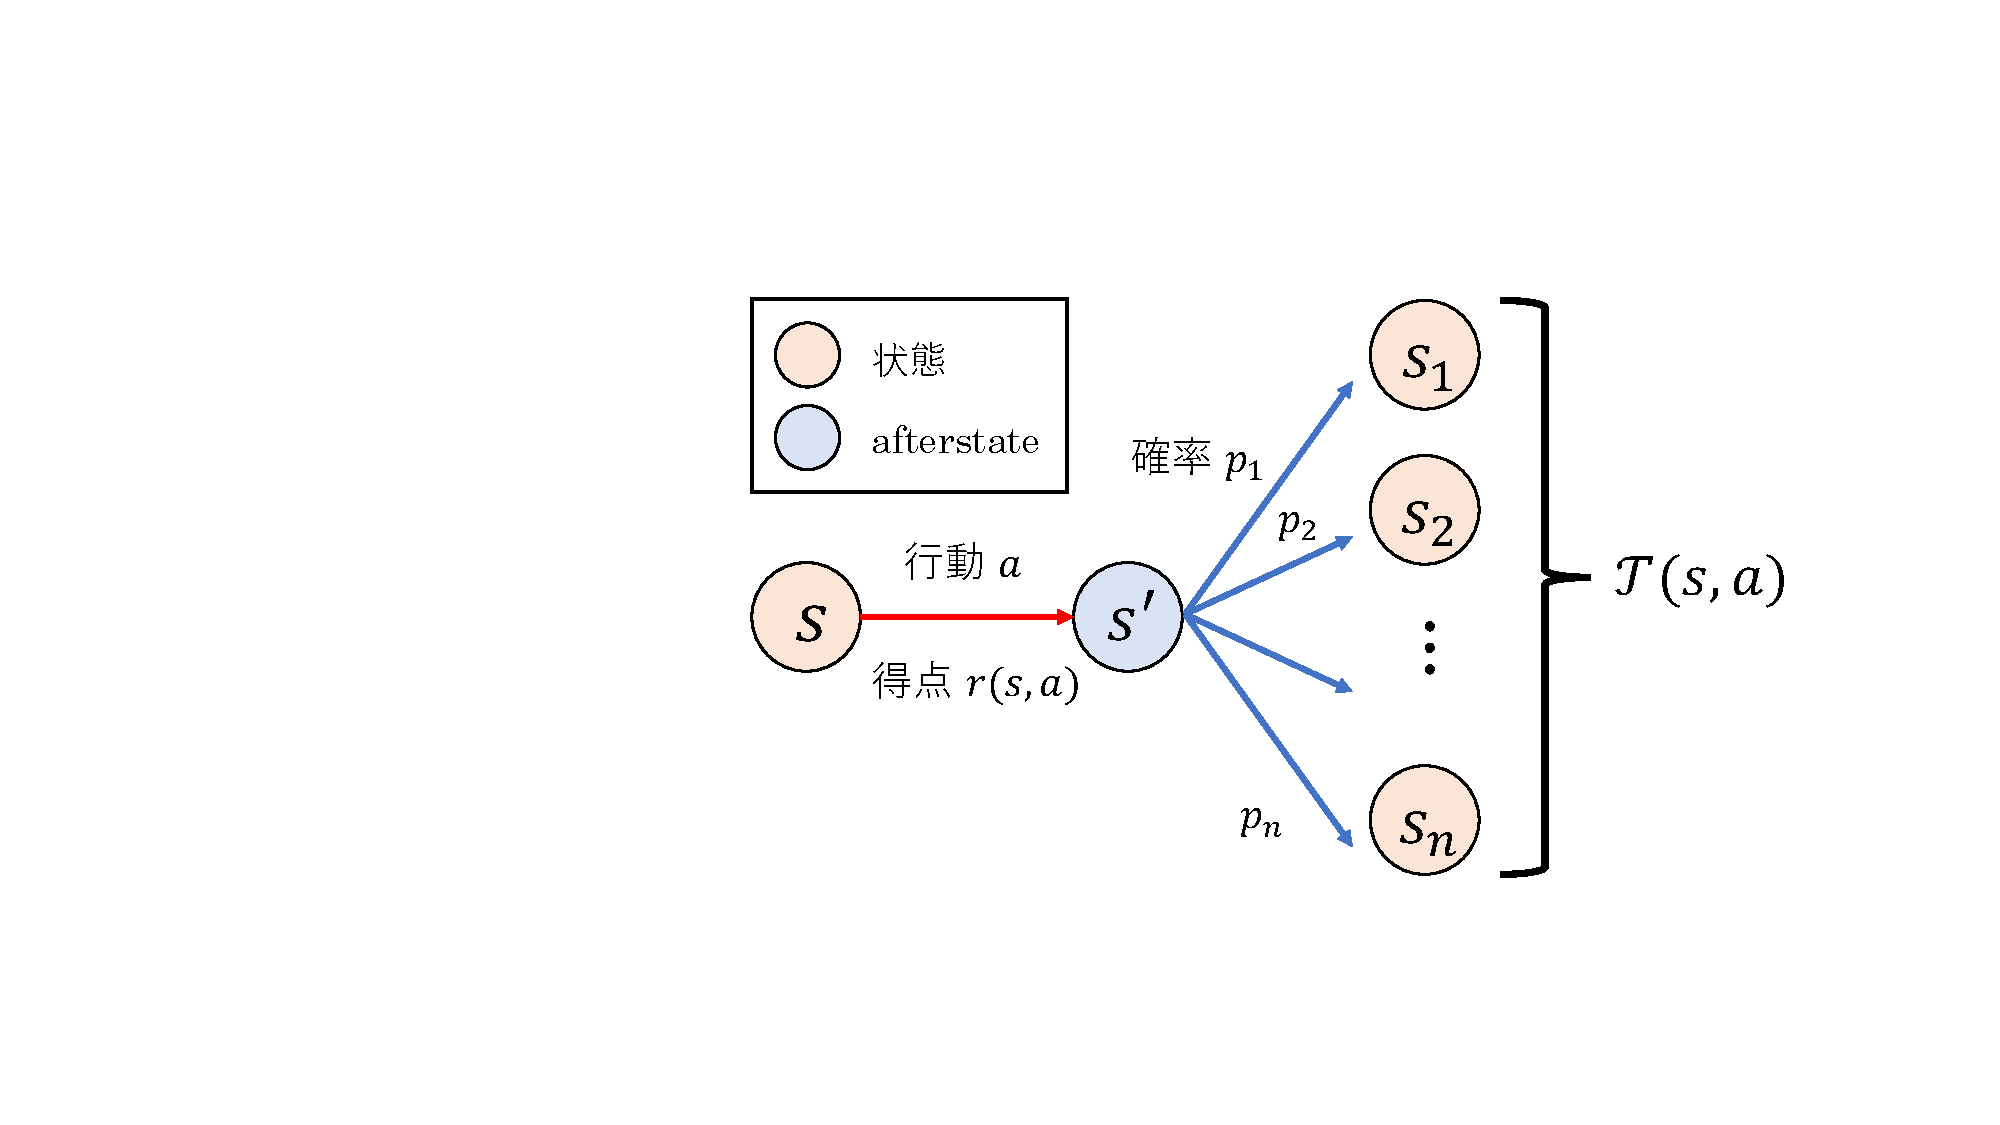
\includegraphics[width=0.6\linewidth{}]{figures/value_function_.pdf}
    \caption{式~\ref{eq:value}の補足図}
    \label{fig:state_afterstate}
\end{figure}

ゲームに現れうるすべての状態の最適価値を計算すれば, 任意の状態において最善手を選ぶことができる.
本稿ではこれを2048の完全解析ということにする.

完全解析をすることで, ゲームの任意の状態の最適価値・最善手を明かし, 最善手を選び続けるプレイヤの戦略を解析することができる.
さらに2048を対象とした強化学習手法の良し悪しを定量的に評価し, より良い手法を提案することができると考えられる.
一方で2048を完全解析することは, そのゲーム木の大きさによる計算コストの観点から現状難しいと考えられる.
そこで本来$4\times4$盤面上で行われる2048のミニゲームとして, 盤面サイズを縮小した2048を完全解析することを考える.

\subsection{盤面サイズが小さな2048の完全解析}
\label{sec:mini2048}
基本的なルールは2048と同じで盤面サイズを$4\times4$から縮小したゲームを完全解析することを考える.
盤面サイズに関わらず, 以下の$2$つのステップを順番に行うことで2048を完全解析することができる.

\begin{enumerate}
    \item ゲームに現れうるすべての状態の列挙
    \item 列挙した状態の価値の計算
\end{enumerate}

\ref{subsec:enumeration}節と~\ref{subsec:calculation}節で具体的な方法について述べる.
なお本節の内容は文献~\cite{3x3_2048}および文献~\cite{4x3_2048}を元に執筆された.

\subsubsection{幅優先探索によるすべての状態の列挙}
\label{subsec:enumeration}
完全解析の第1ステップとして幅優先探索によってゲームに現れうるすべての状態を列挙する.
まず初期状態をキューに詰めて探索を開始する.
キューの先頭の状態$s$を取り出し, $s$から遷移可能な次の状態$s_{\text{next}} \in \mathcal{T}(s)$をキューに追加する.
これをキューが空になるまで繰り返すことで, すべての状態を列挙することができる.

ここで$s_{\text{next}} \in \mathcal{T}(s)$がすでに発見済みであるか確認するために, これまでに発見した状態を管理する集合が必要である.
素朴な方法ではメモリでこれまでに発見した全状態を管理することで行えるが, 状態数が非常に大きな場合にはメモリの容量を超えてしまう.

そこで~\ref{sec:property}節で説明した時刻によってゲーム木を整理する.
時刻$t$の状態は時刻$t+2$か$t+4$の状態にしか遷移しないため, 時刻$t+2$と$t+4$の発見した状態をメモリで管理すれば十分である.
よって時刻が最小の$4$の状態から時刻$2$刻みで順番に列挙を行うことで, ディスクを効率的に活用することができる.
以上を踏まえた疑似コードをAlgorithm~\ref{alg:bfs}に示す.

\begin{algorithm}[tb]
\caption{幅優先探索によるすべての状態の列挙}
\label{alg:bfs}
\begin{algorithmic}[1]
\Function {enumeration}{}
    \For {$t=4$ to $t_{max}$}
        \ForAll {$s_t \in \text{queue}_t$} 
            \ForAll {$s_{t+2} \in \mathcal{T}(s_t)$}
                \State $\text{queue}_{t+2}.\text{push}(s_{t+2})$
            \EndFor
            \ForAll {$s_{t+4} \in \mathcal{T}(s_t)$}
                \State $\text{queue}_{t+4}.\text{push}(s_{t+4})$
            \EndFor
        \EndFor
    \EndFor
\EndFunction
\end{algorithmic}
\end{algorithm}

\subsubsection{後退解析による状態の価値の計算}
\label{subsec:calculation}
\ref{subsec:enumeration}節で列挙した状態の価値を式~\ref{eq:value}に従って計算する.
時刻$t$の状態の価値は, 時刻$t+2$と$t+4$の状態の価値が計算済みであれば計算できる.
よって時刻が最大の状態から順番に走査することで, 効率的にすべての状態の価値を計算できる.
疑似コードをAlgorithm~\ref{alg:calculation}に示す.

\begin{algorithm}[tb]
    \begin{algorithmic}[1]

    \Function {calculation}{$t$}
        \For {$t=t_{max}$ to $4$}
            \State $v(s) = \max_a \left(r(s,a) + \mathbb{E}_{s_\text{next} \in \mathcal{T}(s,a)} v_*(s_\text{next}) \right)$
        \EndFor
        \ForAll {$s_t \in \text{queue}_t$} 
            \ForAll {$s_{t+2} \gets s_t$}
                \State $\text{queue}_{t+2}.\text{push}(s_{t+2})$
            \EndFor
            \If {$element > max$}
                \State $max \gets element$
            \EndIf
        \EndFor
        \State \Return $max$
    \EndFunction
    \end{algorithmic}
    \caption{後退解析による価値計算}
    \label{alg:calculation}
\end{algorithm}

\subsection{実験結果}
$2\times2$盤面から$4\times3$盤面までの2048を完全解析した結果を表~\ref{table: analysis_table}に示す.
\begin{table}[t]
    \centering
    \begin{tabular}{rrr}
        \hline \hline
        盤面サイズ & 状態数 & 初期状態の価値\\ \hline
        $2\times2=4$ & $110$ & $67.6$ \\
        $3\times2=6$ & $21,752$ & $480.9$ \\
        $4\times2=8$ & $4,980,767$ & $2,642.6$ \\
        $3\times3=9$ & $48,713,519$ & $5,469.2$ \\
        $4\times3=12$ & $1,152,817,492,752$ & $50,724.2$ \\
        \hline
    \end{tabular}
    \caption{盤面の大きさと解析結果に関する表}
    \label{table: analysis_table}
\end{table}
盤面サイズが大きくなるに従って指数関数的に状態数は大きくなることが分かる.
また初期状態の価値は, 盤面サイズが$n$マス増える度に$2^n \sim 2^{n+1}$倍になっていることが分かる.
そのため$4\times4$盤面の2048は完全解析を行うには状態数が非常に大きく, 初期状態の価値は約$800,000$点程度ではないかと予想される.

$3\times3$盤面と$4\times3$盤面の2048の各時刻における状態数のグラフを図~\ref{fig:state_afterstate}に示す.
多くのゲームでは進行に従って多様な盤面が存在するため状態数は大きくなり続ける.
一方で2048は盤面が数字タイルで埋まるとゲームオーバーになりやすく, その時刻の状態数は少なくなる.
大きな数字タイルを完成させると盤面上に空きマスが増え, ゲームは再び複雑性を増す.
実際, 図~\ref{fig:state_afterstate}からは$2^n$の前後の時刻で状態数が大きく増減していることが見て取れる.
よって2048はゲームの進行に従って, ゲームの複雑性が増減するという特徴を持つ.
このため任意の時刻における状態数は一定の上限で抑えられ, ~\ref{subsec:enumeration}節と~\ref{subsec:calculation}節で説明した完全解析を実行できる.
\begin{figure}
\vspace{0.2cm}
\begin{subfigure}[T]{0.3\columnwidth}
    \centering
    \includegraphics[width=\columnwidth]{figures/graph_mini_.pdf}
    \caption{$3\times3$盤面の2048}
    \label{fig:graph_mini}
\end{subfigure}
\begin{subfigure}[T]{0.3\columnwidth}
    \centering
    \includegraphics[width=\columnwidth]{figures/graph_mid_.pdf}
    \caption{$4\times3$盤面の2048}
    \label{fig:graph_mid}
\end{subfigure}
\begin{subfigure}[T]{0.3\columnwidth}
    \centering
    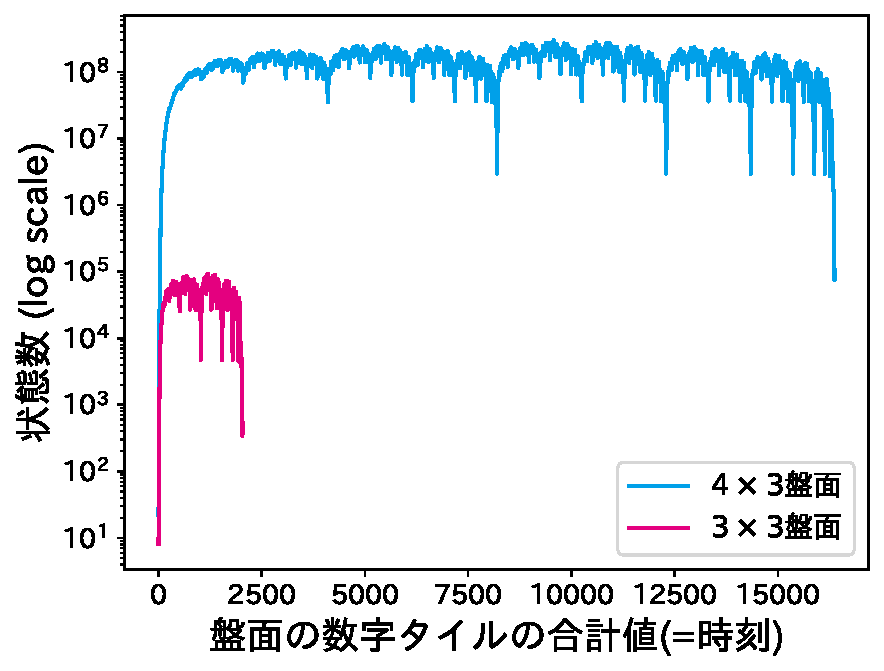
\includegraphics[width=\columnwidth]{figures/graph_compare_mid_mini_.pdf}
    \caption{$3\times3$盤面と$4\times3$盤面の状態数の比較}
    \label{fig:graph_compare_mid_mini_}
\end{subfigure}
\caption{時刻と状態数のグラフ}
\label{fig:time_state_num}
\end{figure}

参考として, $2\times2$盤面の2048のゲーム木全体を図~\ref{fig:game_tree}に示す.
ゲーム木が増大と縮小を繰り返す様子が見て取れる.
\begin{figure}[t]
    \centering
    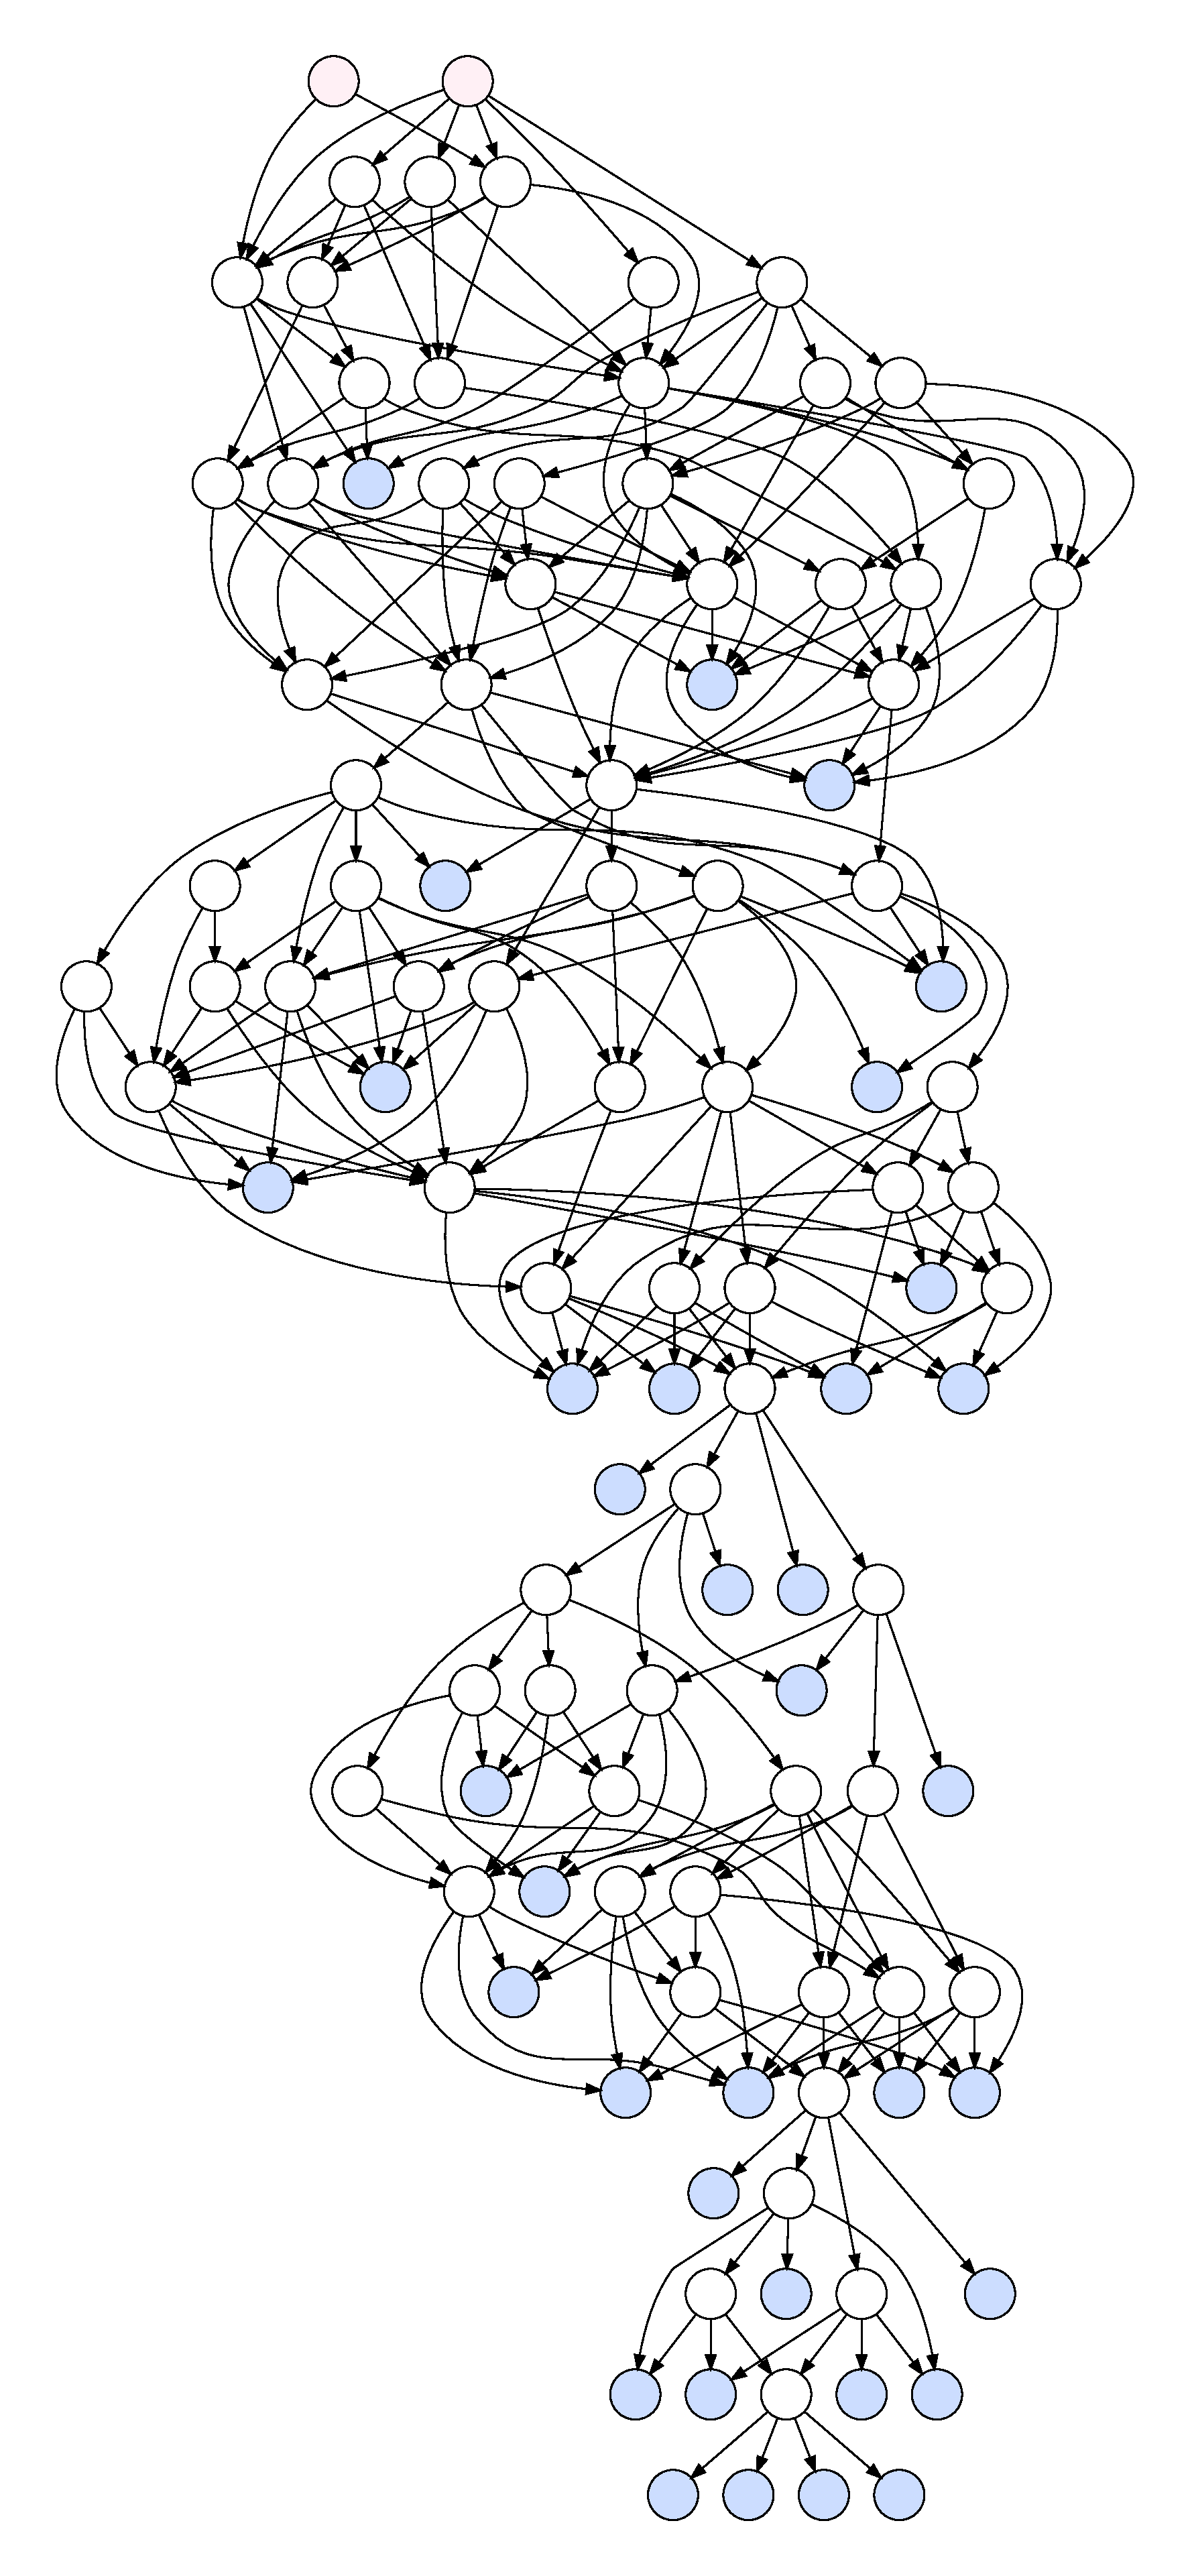
\includegraphics[width=0.7\linewidth{}]{figures/tree.pdf}
    \caption{$2\times2$盤面の2048のゲーム木~(赤色のノードは初期状態, 青色のノードは終了状態)}
    \label{fig:game_tree}
\end{figure}

\appendix
\chapter{実装の詳細}

\section{ゲーム環境の実装}
2048は状態からafterstateへの遷移において, 各行~(列)~の変化は独立に考えることができる.
また回転と反転を考慮することで上下左右は等価な盤面変化を起こす.
よって$1$行の全パターンについて, ある一方向を選択したときの遷移先を前もって計算することで, 全方向に対する盤面全体の遷移を高速に行える.

\section{完全解析の実装}
回転・反転に関して同じ盤面は$1$つの状態として扱った.
またそれぞれの状態は$64$ビット整数で表現された.

$3\times3$盤面の2048の完全解析は状態列挙, 価値計算

\section{強化学習の実装}
\subsection{ニューラルネットワークの詳細}
ニューラルネットワークは盤面の特徴量を入力として, 方策と価値を出力する.
盤面サイズ$H \times W$のルールの下では理論上の最高到達タイルは$2^{H \times W + 1}$である.
このとき入力は空きマス$H \times W + 2$チャネルの$H \times W$から成る.
$n$番目のチャネルの$(i,j)$成分には盤面の$(i,j)$
\begin{figure}[t]
    \centering
    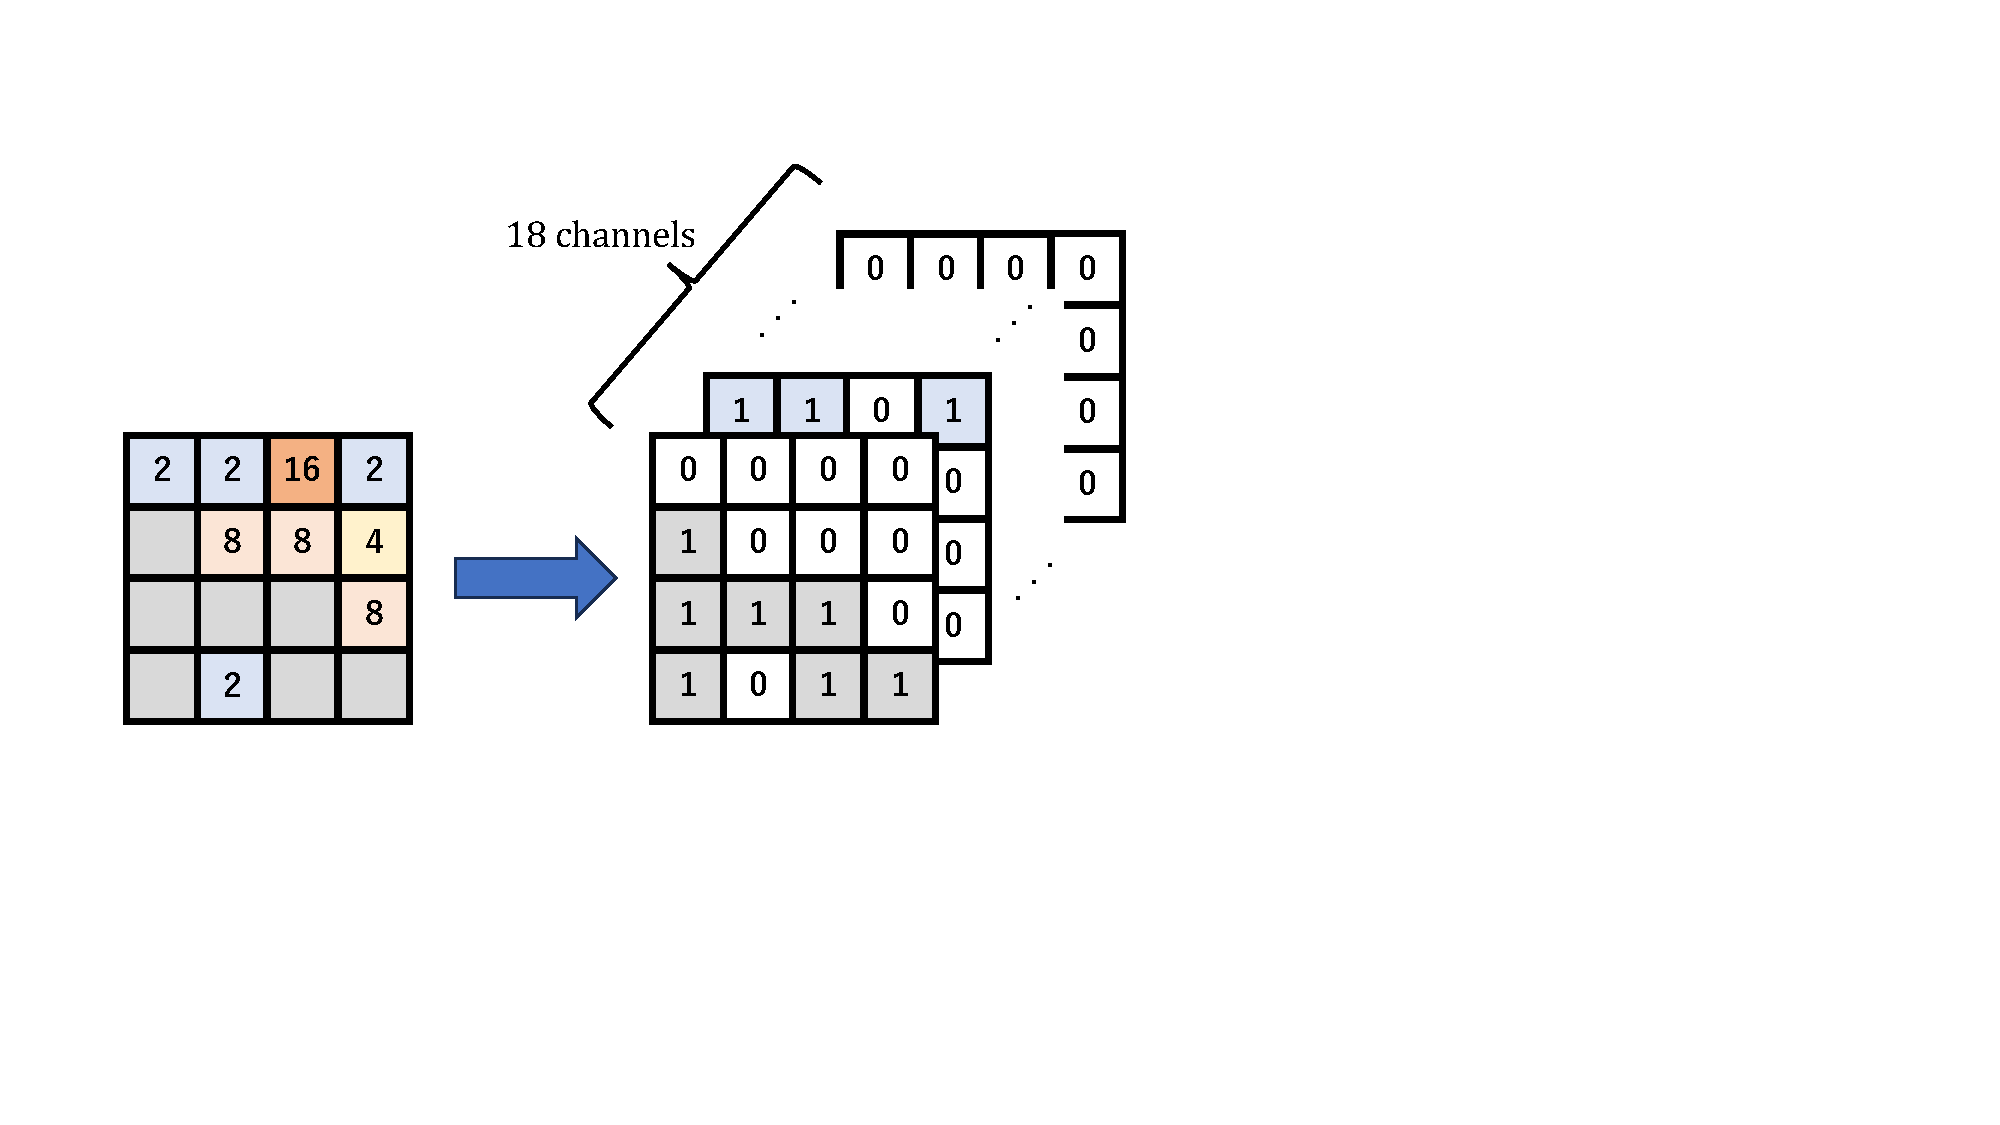
\includegraphics[width=0.6\linewidth{}]{figures/encoding.pdf}
    \caption{ニューラルネットワークへの入力特徴量}
    \label{fig:input_encoding}
\end{figure}

またStochastic MuZero~\cite{StochasticMuZero}に倣って, ニューラルネットワークは価値を$D$次元のベクトル値として出力する.
価値の学習ターゲット$x$~(スカラー値)~は, まず$h(x)= \sqrt{x+1} - 1 + \epsilon x \ (\epsilon=0.001)$によってスケールを調整する~(図~\ref{fig:transform}を参照).
\begin{figure}[t]
    \centering
    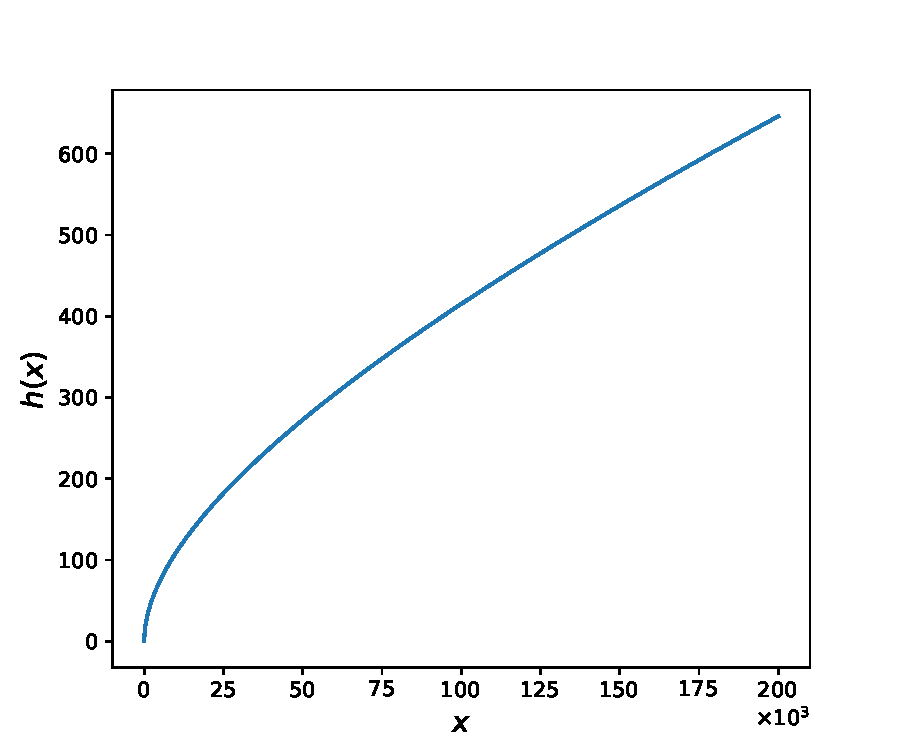
\includegraphics[width=0.6\linewidth{}]{figures/transform_.pdf}
    \caption{$h(x)$のグラフ}
    \label{fig:transform}
\end{figure}
さらに$h(x)$はtwo-hotという, 特定の$2$つの要素以外は全ての$0$であるようなベクトル値に変換される.
たとえば$h(x)=3.7$の場合, $3.7=3 \times 0.3 + 4 \times 0.7$であるため, $3$の重みが$0.3$, $4$の重みが$0.7$, それ以外は$0$である$D$次元ベクトルに変換される.
これをニューラルネットワークの価値の学習ターゲットとして, Cross Entropy誤差を最小化するように訓練される.
推論時にはニューラルネットワークの価値の出力を, softmaxにより全体の総和を$1$にする.
これを$0$から$D$までのそれぞれの重みとして, 重み付け平均$y$を計算する.
最後に$h(x)$の逆関数である$h^{-1}(y)= \epsilon^{-1} (y + 0.5\epsilon^{-1} + 1.0) - 0.5 \sqrt{4.0 \epsilon^{-3} y + 1.004 \epsilon^{-4}}$によって, $x=h^{-1}(y)$を得る.
$3\times3$盤面の2048の実験では$D=200$, $4\times3$盤面では$D=400$, $4\times4$盤面では$D=600$とした.

\subsection{AlphaZeroのニューラルネットワーク}
ニューラルネットワークが出力する価値は, 
ニューラルネットワークは入力に対して方策と価値を出力する.
方策は上下左右それぞれの方向を選択する確率を表す$4$次元のベクトル値である.
価値をベクトル値として出力する.
価値の

\subsection{Prioritized Experience Replayの実装}
Prioritized Experience Replay~\cite{prioritized}は学習に使用するデータを一様ランダムではなく, priorityと呼ばれる重みに従ってサンプルするリプレイバッファである.
リプレイバッファの$i$番目のデータのpriorityを$p_i$とする.
このとき$i$番目のデータはハイパーパラメータ$\alpha$を用いて, 確率$P(i) = \frac{p_{i}^{\alpha}}{\Sigma_k p_{k}^{\alpha}}$でサンプルされる.

Prioritized Experience Replayからのデータのサンプル, およびpriorityの更新は, sum-treeという二分木でデータを管理することで$\mathcal{O}(\log n)$で行うことができる.
sum-treeの葉ノードはpriorityの値を保持し, 各ノードは左右の子ノードの合計値を保持する.
そのため根ノードはpriority全体の合計値$S$を持つ.
サンプルする際には, まず$0$から$S$までの値をランダムに生成し, 根ノードから葉ノードに至るまでたどることで選ぶ.
図~\ref{fig:sumtree}にsum-treeと具体的なサンプルの仕方を例示する.
\begin{figure}[t]
    \centering
    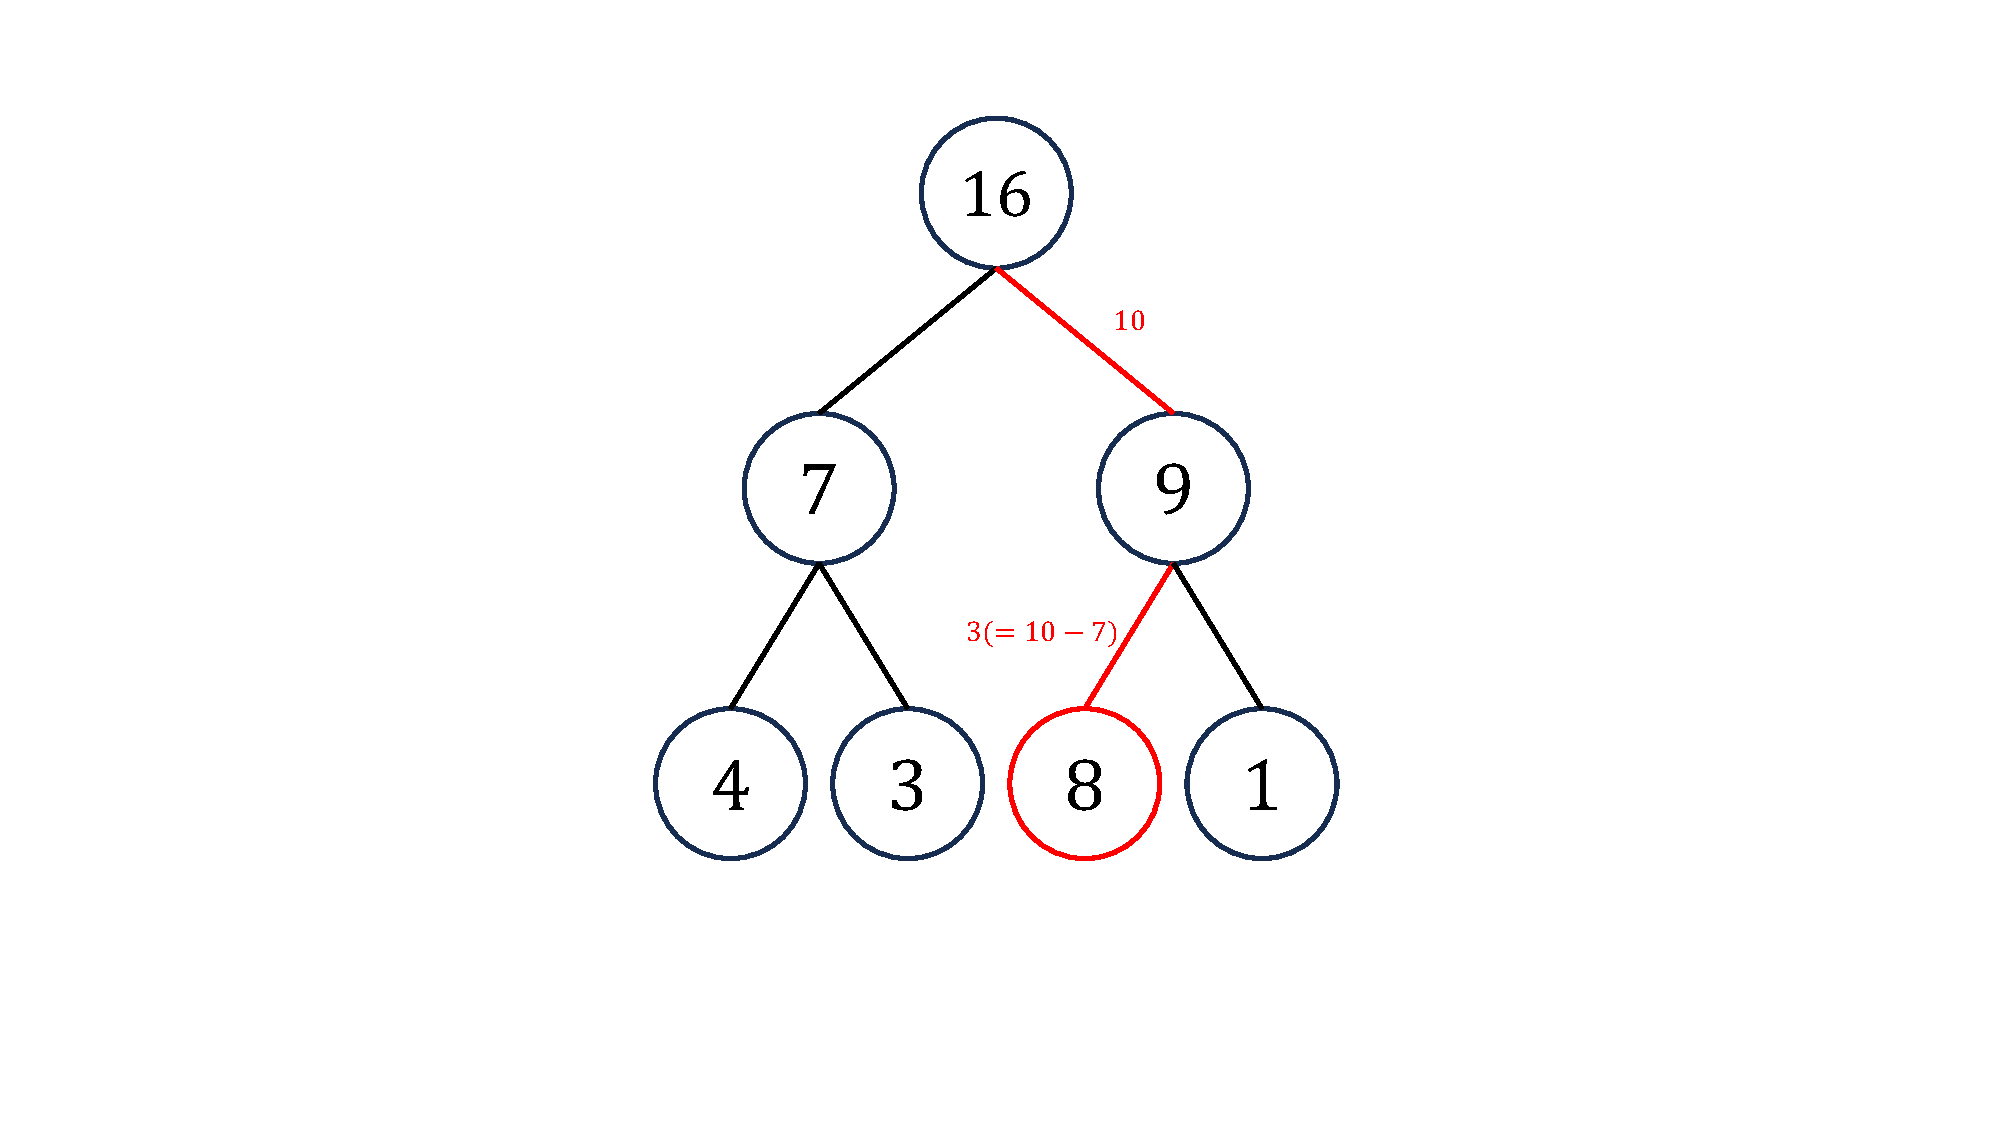
\includegraphics[width=0.4\linewidth{}]{figures/sumtree_.pdf}
    \caption{sum treeの例}
    \label{fig:sumtree}
\end{figure}

\chapter{2048のゲーム性とプレイヤの戦略の検証}
\ref{sec:rule}節で述べたように, 2048の通常のルールではafterstateが次の状態へ遷移する際に出現する, 新しいタイルの数字と位置はランダムに決まる.
すなわちafterstateの空きマスから等確率に選択されたある1マスに$90\%$の確率で$2$のタイルが, $10\%$の確率で$4$のタイルが置かれる.

ここで$2$のタイルと$4$のタイルの出現確率を変更した場合にゲーム性がどう変わるか検証する.
表~\ref{table: value_table}に$3 \times 3$盤面の2048において, $4$の出現確率を通常の$10\%$から増減させたときの完全解析の結果を示す.
表から分かるように, $2$と$4$の出現確率がいずれか一方に傾くほど期待値は大きくなる傾向があることが分かる.
また$4$の出現確率が$0\%$の場合と$100\%$の場合には, 最適な行動をし続ければ常に~図\ref{fig:limit}のような理論上の最終盤面に到達できることが分かる.
2048は$2$と$4$の$2$種類の数字タイルが出現することがゲームを面白くしていると考えられる.
\begin{table}[t]
\caption{4の出現確率を増減させたときのゲームの期待値}
\label{table: value_table}
\centering
\begin{tabular}{r|r||r|r}
    \hline 
    4の確率 & 初期状態の期待値 & 4の確率 & 初期状態の期待値 \\ \hline \hline
    0.00 & 7172.00 & 0.55 & 3206.00 \\
    0.05 & 6161.17 & 0.60 & 3171.24 \\
    \textbf{0.10} & \textbf{5468.49} & 0.65 & 3165.36 \\
    0.15 & 4932.54 & 0.70 & 3194.44 \\
    0.20 & 4515.42 & 0.75 & 3269.18 \\
    0.25 & 4182.44 & 0.80 & 3399.20 \\
    0.30 & 3919.20 & 0.85 & 3607.78 \\
    0.35 & 3704.44 & 0.90 & 3993.30 \\
    0.40 & 3531.46 & 0.95 & 4938.20 \\
    0.45 & 3390.19 & 1.00 & 14344.00 \\
    0.50 & 3278.70 &  & \\
    \hline
\end{tabular}
\end{table}

さらに環境が常にプレイヤにとって最も都合の悪くなるように, 新しい数字タイルを出現させるゲームを考える.
これは得点を最大化したいプレイヤと得点を最小化したい環境の対戦ゲームのように考えることができる.
そのため二人零和有限完全確定情報ゲームと同様に, minmax法によってすべての状態の価値$v_{\text{minmax}}$を計算することができる.
具体的には以下の式~\ref{eq:minmax}に従って, ~\ref{sec:solving}節と同様に後退解析を行えばよい.
環境にランダム性がないため, $v_{\text{minmax}}$は常に固定の値をとる.
\begin{align}
    v_{\text{minmax}}(s) =
    \begin{cases}
        0 & (s \text{が終了状態}) \\
        \max_a \left(r(s,a) + \min_{s_\text{next} \in \mathcal{T}(s,a)} v_{\text{minmax}}(s_\text{next}) \right) & (\text{otherwise})
    \end{cases}
    \label{eq:minmax}
\end{align}

さらに$v_{\text{minmax}}$を評価関数として, 通常のルールでプレイさせることを考える.
悲観的な
よってこれをminmaxプレイヤと呼ぶことにする.
一方で常に都合の良い場合を想定して行動する楽観的な戦略も考えられる.
minmaxプレイヤと対比して, これをmaxmaxプレイヤと呼ぶことにする.

次に

\bibliography{ref} % 研究に役に立ちそうならなんでも入れとく
\bibliographystyle{junsrt}

\end{document}